%\documentclass[conference]{IEEEtran}
\documentclass[11pt, a4paper]{article}

\voffset -23 mm
\hoffset -1.5 cm
\newcommand{\carre} { \hfill $\Box$}
\usepackage[dvips]{graphicx}

\renewcommand{\baselinestretch}{1.6}
\headsep=0.0in          %Amount of space between head and top of a page
\evensidemargin=0.1in           %Move right margin half-inch to the right
\textwidth=16.11cm                %Define size of printable area on page
\textheight=23cm
\parskip=1.25ex                 %Amount of space to skip between paragraphs
\parindent=0pt                %Amount of space to indent for a new
                                 %paragraph\footnotesep=3.0ex%\topmargin = 2.5cm
\usepackage{times}
\usepackage{setspace}
\usepackage{subfigure}
\usepackage{latexsym}
\usepackage{amsmath}
\usepackage{amssymb}
\usepackage{epsfig}
%\renewcommand{\baselinestretch}{1.4}

\newtheorem{condition}{\indent \bf Condition}[section]
\newtheorem{property}{\indent \bf Property}[section]
\newtheorem{definition}{\indent \bf Definition}[section]
\newtheorem{conj}{\indent \bf Conjecture}[section]
\newtheorem{cor}{\bf Corollary}
\newtheorem{lemma}{\bf Lemma}
\newtheorem{claim}{\bf Claim}
\newtheorem{theorem}{\bf Theorem}
\newtheorem{prop}{\indent \bf Proposition}[section]
\newtheorem{remark}{\indent \bf Remark}[section]
%\newenvironment{proof}{\indent {\bf Proof:}}{\hfill$\bf \Box$\bigskip}
%\newenvironment{proofl}{\indent {\bf Proof of Lemma }}{\hfill$\bf %\Box$\bigskip}
%\newenvironment{prooft}{\indent {\bf Proof of Theorem }}{\hfill$\bf \Box$\bigskip}
\newenvironment{example}{\indent {\bf Example:}}{\hfill$\bf \Box$\bigskip}
\markright{Brampton et al. \hfill \today\hfill }

\begin{document}
%\doublespacing
%\graphicspath{{:EPS:}{:}{./EPS/}{./}}
\title{Nodes authentication in Stealth DHT}
%\date{}
\author{Andrew Brampton, Andrew MacQuire, Idris A. Rai, Nicholas J. P. Race and Laurent Mathy\\
Computing Department\\
Lancaster University\\
{\{brampton,macquire,rai,race,laurent\}@comp.lancs.ac.uk}}
\maketitle
% placeholder abstract to replace ugly x's :)
\begin{abstract}

\end{abstract}

\section{Introduction}
\label{sec1}

\section{Overview of Stealth DHT}
\label{stealth}

\section{The need for nodes authentication in Stealth DHT}

\section{Overview of Public key infrastructure}
%- Define -components/building blocks -functions/uses
%-implementations considerations

A {\em public key infrastructure} (PKI) it is an infrastructure that
uses {\em digital certificates} as an {\em authentication mechanism}
and is built to better manage certificates and their associated
keys. A digital certificate is sometimes called {\em public key
certificate} as it is itself a way to reliably identify the user
claiming to be the owner of a specific public key. In addition,
digital certificates contain information about the {\em identity of
the holder}, the {holder�s public key}, an {\em expiration date of
the certificate}, and the {\em digital signature of the issuer}.


Although PKI derives its name from public key cryptography, some of
the services it provides are far outside the field of cryptography.
In addition to offering authentication mechanisms,  a combination of
secret key and public key cryptography enables  PKI deliver services
including data confidentiality, data integrity, and key management.
The use of digital certificates evolved in asymmetric encryption
because of the difficulty of knowing whether a public key is really
owned by the person it is claimed to belong to. It is possible that
user A advertises that a public key belongs to B when in fact it
doesn't. That user could then intercept messages intended for A and
decrypt them with the private key he has and that belongs to the key
pair. Thus, digital certificates was needed for verifying the
identity of the holder of key pairs. In PKI, it is a trusted entity
called a {\em certification authority} that issues certificates.
Then other users can *rely on the veracity* of the key holder�s
identity.

Managing digital certificates and their associated keys involve a
combination of  complex tasks. In addition to certificate issuance,
PKI was created to provide a framework for the {\em renewal}, {\em
revocation}, and {\em management of certificates}. PKI has a number
of building blocks each of which facilitates a different function of
PKI. The basic building block  is {\em Certification Authority}
(CA). CA is ....... {\em Registration Authority} (RA) is another key
building block, which is concerned with ....... . Finally, {\em
Directory Services} is a building block dealing  with ......

End entities as a PKI building block? see below!

%%---
End Entities or Subscribers: An end entity or subscriber is any user
or thing, including inanimate objects, such as computers that have a
need for a digital certificate to identify them for some reason. The
end entity normally must have the capacity to generate a
public/private key pair and some means of securely storing and using
the private key. By definition, an end entity is not a CA.

Certificate Authorities As noted previously in the discussion on
Trust, a Certificate Authority plays a critical role in a PKI.
According to the IETF, a CA is �an authority trusted by one or more
users to create and assign public key certificates.� [Internet X.509
Public Key Infrastructure PKIX Roadmap, March 10, 2000] To
elaborate, a CA functions as a trusted third party and provides
various key management services. A CA essentially certifies the
identity of an end entity. This is accomplished by an entity
providing sufficient proof of their identity to the CA, and then
having the CA generate a message containing the entity�s identity
and public key. This message is called a certificate and is
cryptographically signed by the CA. The level of trust that a CA has
depends on the level of acceptance that other entities have in that
CA. This level of acceptance depends on the policies and procedures
the CA has established to ascertain the user�s identity. A CA�s
public keys must be distributed to all entities that trust the CA�s
certificates. If a CA is a Root CA, that is, at the top of the trust
hierarchy and has no superior CA to vouch for it, then the CA must
distribute its public keys as self-signed certificates with an
acceptable key certificate format and distribution protocol. The CA
must also make its cleartext public keys available, so that relying
entities can resolve the self-signed certificates. Registration
Authorities A Registration Authority (RA) is an optional but common
component of a PKI. An RA is used to perform some of the
administrative tasks that a CA would normally undertake. Most
importantly, an RA is delegated, with the CA�s explicit permission,
the authority to perform tasks on behalf of the CA. The primary
purpose of an RA is to verify an end entity�s identity and determine
if an end entity is entitled to have a public key certificate
issued. The RA must enforce all policies and procedures defined in
the CA�s CP and CPS. A typical function of an RA is to interrogate
an end entity�s certificate request by examining the name, validity
dates, applicable constraints, public key, certificate extensions,
and related information. The RA may also be responsible for
performing due diligence tests on the end entity. This
responsibility may be as simple as ensuring the name of the end
entity is unique within the scope of the PKI; or, it may be as
involved as making credit checks on potential clients. Certificate
Depositories As with an RA, a certificate depository, sometimes
referred to as a certificate directory, is also an optional but
common component of a PKI. A certificate depository may be an
efficient solution for closed systems (e.g., intranet) or those in
isolated processing environments (e.g., chipcard-based applications)
where the Root CA public key is distributed locally or revocation
lists are stored locally. Many other situations warrant the use of a
certificate or Certificate Revocation List (CRL) depository. The use
of depositories for CRL distribution is discussed later in this
article. Certificate distribution can be accomplished by simply
publishing certificates in a directory controlled by a CA or RA.
When the directory is controlled by the CA or RA, the certificate
distribution process is greatly simplified. Rather than trying to
distribute every certificate to a unique point, the CA simply
updates the directory. A critical factor is that only the CA must
have the authority to update or modify the directory, but the
directory must be publicly readable.

Registration Authorities A Registration Authority (RA) is an
optional but common component of a PKI. An RA is used to perform
some of the administrative tasks that a CA would normally undertake.
Most importantly, an RA is delegated, with the CA�s explicit
permission, the authority to perform tasks on behalf of the CA. The
primary purpose of an RA is to verify an end entity�s identity and
determine if an end entity is entitled to have a public key
certificate issued. The RA must enforce all policies and procedures
defined in the CA�s CP and CPS. A typical function of an RA is to
interrogate an end entity�s certificate request by examining the
name, validity dates, applicable constraints, public key,
certificate extensions, and related information. The RA may also be
responsible for performing due diligence tests on the end entity.
This responsibility may be as simple as ensuring the name of the end
entity is unique within the scope of the PKI; or, it may be as
involved as making credit checks on potential clients. Certificate
Depositories As with an RA, a certificate depository, sometimes
referred to as a certificate directory, is also an optional but
common component of a PKI. A certificate depository may be an
efficient solution for closed systems (e.g., intranet) or those in
isolated processing environments (e.g., chipcard-based applications)
where the Root CA public key is distributed locally or revocation
lists are stored locally. Many other situations warrant the use of a
certificate or Certificate Revocation List (CRL) depository. The use
of depositories for CRL distribution is discussed later in this
article. Certificate distribution can be accomplished by simply
publishing certificates in a directory controlled by a CA or RA.
When the directory is controlled by the CA or RA, the certificate
distribution process is greatly simplified. Rather than trying to
distribute every certificate to a unique point, the CA simply
updates the directory. A critical factor is that only the CA must
have the authority to update or modify the directory, but the
directory must be publicly readable.

LDAP is a good example of a simple and efficient standards based
directory format and protocol that can be used for certificate
distribution. In particular, LDAP is optimized for easy read access
by thin clients that are a necessity in many PKI implementations.
Because LDAP defines an API for the application layer used by
different clients, users realize a level of scalability and
portability, and do not have to contend with the upper layers of the
stack. This API also makes it easier for different applications to
quickly implement LDAP. Although LDAP is becoming a de facto
standard for certificate distribution, organizations that need an
even more robust certificate depository can consider alternatives
such as X.500.

%%-------


In implementing PKI, all building blocks of the PKI can be
incorporated in a  single entity. To distribute the load  among
different entities, some PKI implementations choose to implement the
building blocks in different entities. PKI implementation can also
be termed as either {\em centralized} or {\em decentralized}
(distributed). Centralized PKI ...


% Industry standard
%PKIs and their certificates are built on the X.509 specifications of
%the ISO.

\section{Authentication of nodes in Stealth DHT}
\subsubsection{The Model}
- emphasis to S-DHT but applicable to any DHT,  - CA as a cloud -
 certificate issuing, authenticating - a user / messages

-- Here CA is is assumed as an entity offering all basic functions
of basic  PKI building blocks.


we propose a model where DHT nodes are treated as end entities that
requires to  authenticate other nodes or messages from the a trusted
*organization* (we call it CA or PKI??). Thus nodes makes direct communication
to the organization for any authentication request. The organization
is the entity that manages the PKI. Thus it issues and manages the
certificates of all nodes on the DHT.

====say more what the CA can do? -- a fig needed
\begin{figure}[htb]
% generated using plotjoins.m
\centering 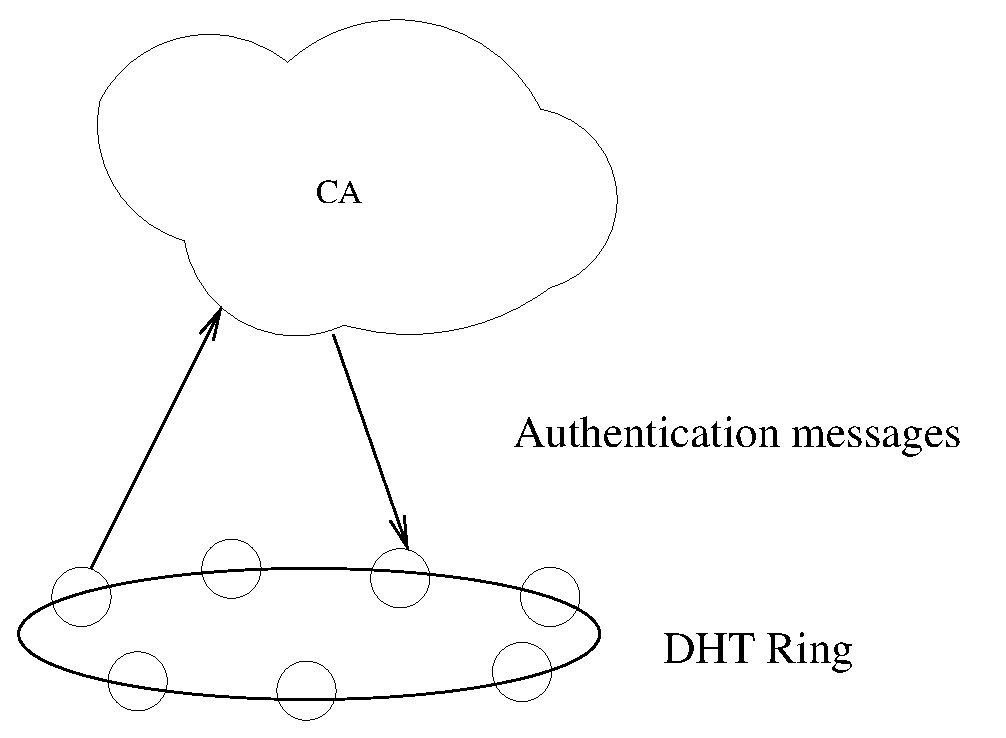
\epsfig{file=mode1.eps, width=0.5\textwidth} \caption{\em
Illustrating the authentication model -- a sample figure}
\label{fig:fg1}
\end{figure}


vendors who will deploy Stealth DHT will be be able to deploy any
authentication infrastructure to offer the required level of
security. the model described in this section the signalling
communication between nodes on DHT, taking the case for Stealth DHT,
to the organization that offers authentication service. The model
doesn't care if the PKI is based on different other entities,
centralized or a distributed entity. It neither cares if the PKI is
within DHT or out of DHT. Although the we propose algorithm for the
former. Thus, the nodes authentication model that we discuss in this
section is in no way bound to the DHT*.

Depending on the required level of security, a node on DHT may wish
to authenticate any of the following: a new node joining the
network, another node that requests a service from it, any message
it is requested to forward, a node who issued a key it is demanded
to store, etc?. In what follows we further discuss how DHT nodes can
use the proposed model in this section  for authentication.

\subsection{Personal Authentication / certificate issuing}
 -- the authentication process starts with personal
registration using any standard method such as username/password,
payment, account number, etc. This  must be done before the join
procedure is executed.

the figure (above) shows interaction between CA and nodes only on
DHT. before a node joins the DHT, it also has to contact the CA for
personal identification and certificate issuing.(explain the
processes) --

say if the node generates its own keys and DHT ID or the CA does
that for him.


\subsection{Secure Joining}

Once registration is complete, a node has its certificate it can use
to securely join the DHT. (explain how this will work in the model).
----He appends the certificate in a join message and each node that
sees the message can independently authenticate the message by
directly  contacting the CA to verify the certificate. ....

% explain the full complete authenticated join procedure here

the message is forwarded only if the authentication is successful
(needed?), (if needed) this will be done for join messages only.

\subsection{Authenticating a node}
The sub-title may be ambiguous here, but the idea is whenever a node
receives a message, say   put or get messages or a message to relay,
that message or (the sender) must be authenticated. Depending on the
level of security demanded, possibilities are that either a message
can be checked per hop or only at the destination. per hop check,
although provides high security level and can eliminate messages
from unauthenticated users on DHT, it incurs high overhead and may
degrade the DHT performance. On the other hand, authentication only
at the destination......

%Say how the messaging overhead affect the DHT performance, in
%general terms.
\subsection{Certificate revocation}
an overview of revocation schemes that exist and that CA can deploy

\section{Distributed PKI in Stealth DHT}
The model above presents an open scenario that does not bind the PKI
to the DHT. In this section, we propose an authentication algorithm
that is fully distributed over the DHT.

notations: Public key $PK$, private key $k$, certificate of a node
X, $C_X$, provider $P$, certificate issuers $I$, service node $S$,
trusted global certificate authority $G$.

What it means by distributed PKI?. - entities or nodes on DHT  can
perform multiple PKI functions, no centralized central authority.
instead, individual nodes can issue, manage, and revoke certificates
themselves. (this must be clearly but completely exaplined)

\subsection{The Model}
The hierarchical model, fig.  The arrow indicates shows the order at
which certificates are issued. Thus the opposite of arrows is the
verification path. tell the components of the model - define G, P,
I, sets of nodes {U} and {S}; the roles of each one in
authentication must be clearly written.

\begin{figure}[htb]
% generated using plotjoins.m
\centering 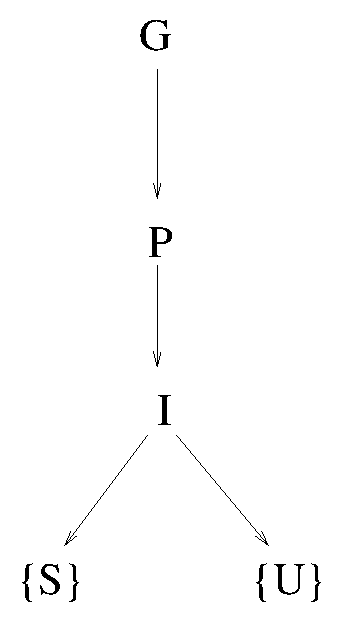
\epsfig{file=mode2.eps, width=0.2\textwidth} \caption{\em
Model Distributed PKI for Stealth DHT -- a sample figure}
\label{fig:fg2}
\end{figure}

 - why need global issuer G, what role plays? -- issuing a
certificate to provider etc etc,

- providers certificate, what is it for, why needed?.

- Issuers, these can be either service nodes on DHT or dedicated
servers away from DHT (pros and cons). what do we propose?


\subsubsection{Secure Joining}
\subsubsection{Authenticating a node}

\section{Revocation}

\section{Experimental results}

\section{Conclusion}

%\nocite{*}
\bibliographystyle{IEEEannot}
\bibliography{authold}
\end{document}
